\section{Experiments}
\begin{figure}[!t]
	\centering
	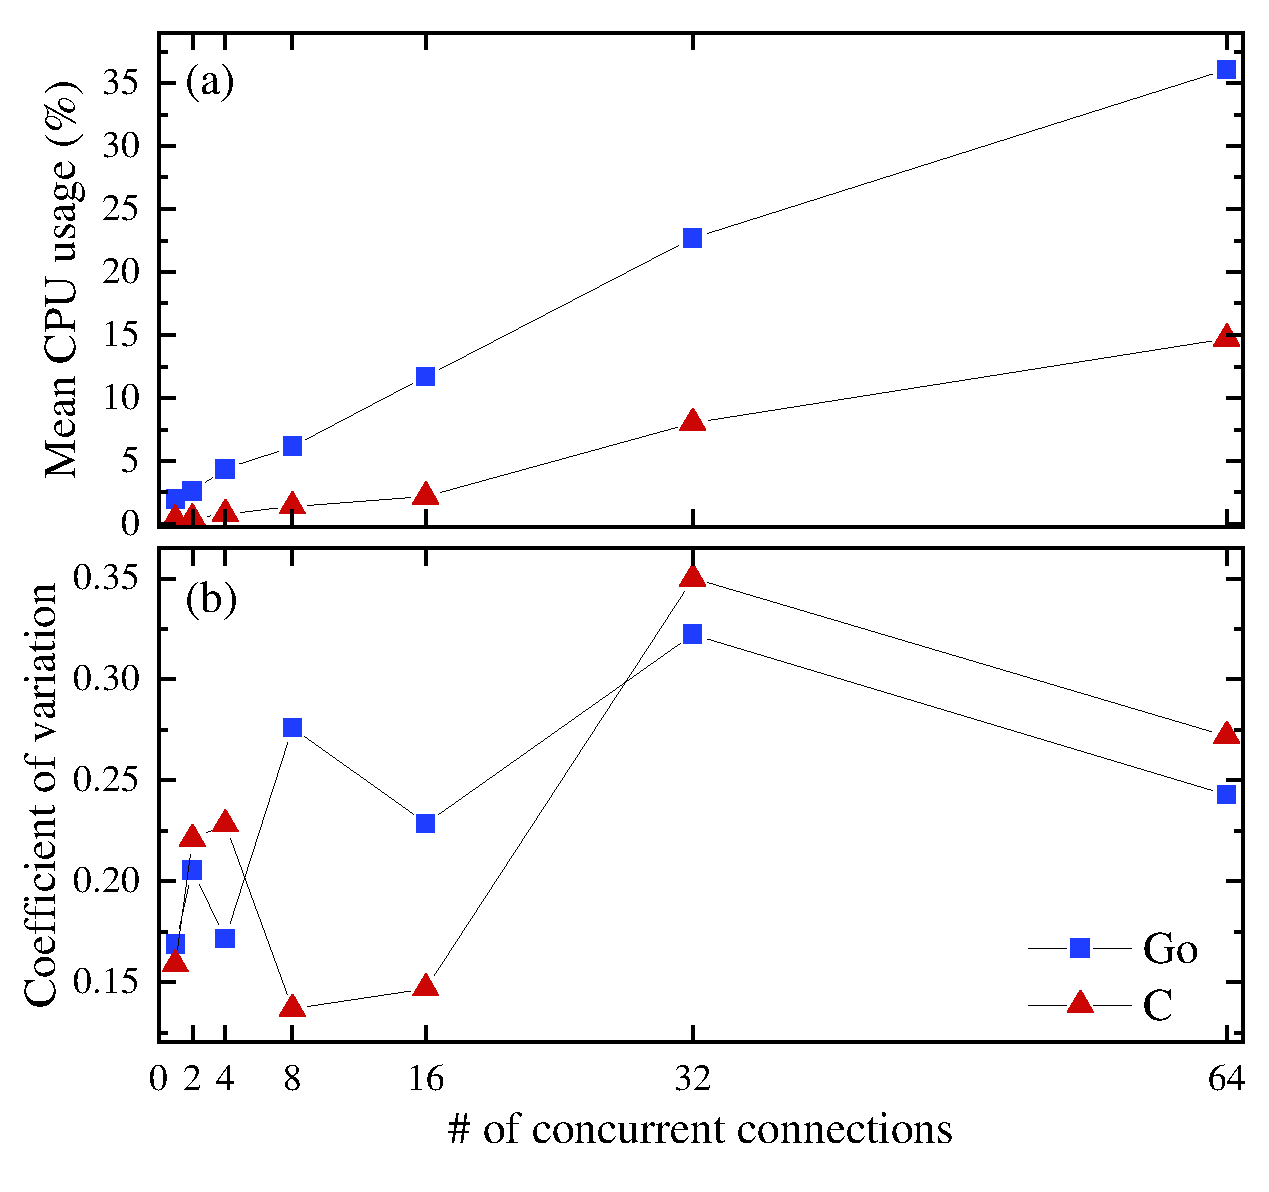
\includegraphics[width=3in]{img/experiments.pdf}
	%where an .eps filename suffix will be assumed under latex, 
	%and a .pdf suffix will be assumed for pdflatex; or what has been declared
	%via \DeclareGraphicsExtensions.
	\caption{(a) compares the mean CPU usage value (\%) in relationship to the number of active concurrent connections. (b) compares the development of the coefficient of variation $C_v$ depending on the number of concurrent connections being handled by the two different concurrency platforms.}
	\label{fig_results}
\end{figure}
To evaluate the performance of a concurrency paradigm based upon context-switching in user-space and another one based upon context-switching in kernel-space, the same very rudimentary IM application was developed in both C and Go. The C program handles concurrent client network connections by spawning a new process per client, while the Go application creates a goroutine for each client. 

% Maybe write, being benchmarked, instead of tested.
A TCP load generator running in a cloud server is used to send a constant load of network packets (1Mbps) per concurrent connection for exactly 60 seconds to another server running the application being tested. Each application accepts a given number of concurrent client connections per test, receives and reads the clients' packets (which simulate text messages coming from the users in a real IM application) and writes the text in the packets to \textit{stdout}. To not overwhelm the system with filesystem writes and focus primarily in the performance of the concurrency-handling mechanisms in a real-life environment, the data being output to stdout is immediately discarded to \textit{/dev/null}. 

The CPU usage of the IM application is measured and recorded using \textit{top(1)} with a sampling rate of 500ms. The number of active concurrent clients is incremented in each new test, starting at 1 and going all the way up to 64 concurrent connections.

\subsection{Test environment}
Both the TCP load generator and the application under test were executed in cloud virtual machines (VM) inside the same region running FreeBSD 13.0-RELEASE-p11 with 1vCPU and 2GB RAM. The versions of software used for these experiments were: for the TCP load generator \textit{tcpkali v1.1.1}, for the C compiler \textit{GCC v10.4} and for the Go compiler \textit{Go v1.18.2}.

\subsection{Constraints}
The cloud VMs were generated exclusively for the tests with the default FreeBSD configuration for a first-time boot, which has a minimal amount of long-running daemons. A small number of system daemons is important to try to interfere with the tests as less as possible. 

Nonetheless, some system daemons were intermittently running during the tests. Especially, \textit{ntpd}, the system daemon in charge of syncing the VM's clock with time servers, recurrently used system resources and forced context-switches when the number of active concurrent clients was low (below 16 active client connections). Running idle, ntpd and the remaining system daemons did not used more than 1,5\% of CPU usage.

%\subsection{Results}
%\begin{table}[h]
%	\centering
%\begin{tabular}{|c|ccr|}
%		\hline
%	\# Conn.         &  Paradigm    & $\mu$ CPU usage [\%] & $\sigma$ $\mu^{-1}$ \\
%	\hline
%	\multirow{2}{*}{1} & C & 0.34 & 0.159   \\
%	&\cellcolor[gray]{0.9} Go &\cellcolor[gray]{0.9} 1.94 &\cellcolor[gray]{0.9} 0.169  \\ \hline
%	\multirow{2}{*}{2} & C & 0.45 & 0.221   \\
%	&\cellcolor[gray]{0.9} Go &\cellcolor[gray]{0.9} 2.61 &\cellcolor[gray]{0.9} 0.205  \\ \hline
%	\multirow{2}{*}{4} & C & 0.79 & 0.228   \\
%&\cellcolor[gray]{0.9} Go &\cellcolor[gray]{0.9} 4.35 &\cellcolor[gray]{0.9} 0.172  \\ \hline
%	\multirow{2}{*}{8} & C & 1.37 & 0.137   \\
%&\cellcolor[gray]{0.9} Go &\cellcolor[gray]{0.9} 6.15 &\cellcolor[gray]{0.9} 0.276  \\ \hline
%	\multirow{2}{*}{16} & C & 2.17 & 0.147   \\
%&\cellcolor[gray]{0.9} Go &\cellcolor[gray]{0.9} 11.71 &\cellcolor[gray]{0.9} 0.229  \\ \hline
%	\multirow{2}{*}{32} & C & 2.53 & 0.172   \\
%&\cellcolor[gray]{0.9} Go &\cellcolor[gray]{0.9} 22.71 &\cellcolor[gray]{0.9} 0.322  \\ \hline
%	\multirow{2}{*}{64} & C & 2.53 & 0.180   \\
%&\cellcolor[gray]{0.9} Go &\cellcolor[gray]{0.9} 36.08 &\cellcolor[gray]{0.9} 0.243  \\ \hline
%\end{tabular}
%\bigskip	
%\caption{The table shows a comparison of the mean ($\mu$) CPU usage in \% and the coefficient of variation of the CPU usage $\frac{\sigma}{\mu}$ measured on the IM rudimentary application with a multi-process concurrency paradigm (C) and a non-preemptive scheduler (Go) under a load of a different number of concurrent network connections (\# Conn.).}
%\label{tab_results}
%\end{table}

%% TODO: create a new graphic that integrates both C and Go measurement with 2 clients.